\documentclass{article}

\usepackage[preprint]{neurips_2026}

\usepackage[utf8]{inputenc}
\usepackage[T1]{fontenc}
\usepackage{hyperref}
\usepackage{url}
\usepackage{booktabs}
\usepackage{amsfonts}
\usepackage{nicefrac}
\usepackage{microtype}
\usepackage{xcolor}
\usepackage{graphicx}
\usepackage{amsmath}
\usepackage{amssymb}
\usepackage{mathtools}
\usepackage{bm}
\usepackage{multirow}

\title{TailFlow: Inference-Time Noise Scaling Is Sufficient\\
for the Body--Tail Trade-off in One-Step Probabilistic Forecasting}

\author{Anonymous Authors}

\begin{document}

\maketitle

\begin{abstract}
Probabilistic time-series forecasters have to make a trade-off between
central calibration (how well $90\%$ prediction intervals cover the data)
and upper-tail sharpness (how accurately probability mass is placed on
rare large values). The recent twCRPS-weighted training approach of
Wessel et al.\ (2025) makes this trade-off a \emph{training} choice:
different thresholds $\tau$ yield different fine-tuned models, each
locked into one body--tail operating point, each requiring a separate
training run. We show that on a strong one-step S4D-MeanFlow backbone
this trade-off can instead be traced out at inference time by a single
scalar: the Gaussian noise scale $n$ at the starting point of the
one-step flow sampler. A single trained model reaches the
\emph{same} body--tail Pareto frontier as a family of three twCRPS-retrained
variants on solar, at zero retraining cost. Our one-NFE base also
matches or beats TSFlow (ICLR 2025) on central calibration (CRPS),
central-PI coverage, and 95\% Winkler interval score on all four NIPS4
benchmarks under uniform scoring we re-implemented (with threshold-
weighted CRPS thresholds computed correctly from the training marginal
distribution, following Allen et al.\ JASA 2025), while using
$32\times$ fewer forward passes at inference and giving
$32\times$ lower wall-clock latency on matched backbones. On a
heavy-tailed air-quality dataset (KDD Cup 2018, kurtosis $\approx 35$)
TailFlow halves bootstrap's $95\%$ Winkler score with correct coverage.
TSFlow retains a genuine advantage on solar upper-tail twCRPS at
$\tau{=}0.99$ via its Gaussian-process prior; we report this honestly
and sketch an extension that combines the GP prior with our
inference-time dial.
\end{abstract}

\section{Introduction}
\label{sec:intro}

Many practical forecasting applications care about both body and tail
calibration simultaneously: grid operators need accurate central
day-ahead forecasts for dispatch \emph{and} well-sized peak-demand
scenarios for reserve planning, air-quality regulators need both
typical-day forecasts \emph{and} pollution-spike warnings, and risk
managers need point estimates \emph{and} tail-scenario stress tests.
The standard probabilistic-forecasting objective (Gneiting CRPS) is
optimized for central calibration, which leaves the upper tail
under-covered, and training-time twCRPS reweighting of
Wessel et al.~\cite{wessel2025tail} improves tail sharpness only at the
cost of either body calibration or a separate retraining pass for
each operating point.

\paragraph{Key observation.} A one-step MeanFlow sampler
$\hat{z}_0 = z_1 - u(z_1, t{=}1, h{=}1, \text{context})$ with
$z_1 \sim \mathcal{N}(0, n^2 I)$ uses a single scalar $n$ to fix the
variance of its starting distribution. Training uses $n=1$, but the
same trained velocity field $u$ at inference time can be fed samples
from any $n>0$. Because the training distribution of normalized solar
futures has peak-to-mean ratios far in excess of what $\mathcal{N}(0, I)$
typically produces, \emph{widening the starting prior at inference is
necessary for the sampler to reach the tail of the data distribution
at all}, and \emph{the scale of the widening directly controls where
the sampler sits on the body--tail Pareto frontier}.

\paragraph{Central claim.} On a strong one-step S4D-MeanFlow backbone,
inference-time noise scaling is \emph{sufficient}: it matches the best
operating points reached by training-time twCRPS reweighting on solar
at every threshold $\tau \in \{0.90, 0.95, 0.99\}$, using a single
trained model instead of a retrained family. Crucially, \emph{we do
not claim} that our dial is fundamentally more expressive than
retraining; we claim it is \emph{as expressive}, and therefore
strictly cheaper.

\paragraph{Contributions.}
\begin{enumerate}
\item We empirically characterize the inference-time noise scale $n$
as a continuous dial over body CRPS vs upper-tail twCRPS on a strong
one-step MeanFlow backbone. One trained model is scored at five values
of $n$; the resulting curve matches the best twCRPS-retrained variants
on solar within sampling noise (Figure~\ref{fig:pareto}).
\item We reimplement a uniform tail-metric evaluation
(\texttt{meanflow\_ts/tail\_metrics.py}) that computes threshold-weighted
CRPS with train-distribution thresholds (not test-set thresholds, which
are improper; see \S\ref{sec:metrics}), and re-evaluate TSFlow
(Kollovieh et al.\ ICLR 2025) from the official repository under this
code. We report both the bulk CRPS leaderboard and the full tail
table (twCRPS$_{0.95}$, twCRPS$_{0.99}$, coverage, Winkler$_{0.95}$)
for solar, electricity, traffic, exchange rate, and KDD Cup 2018.
\item We measure wall-clock inference latency: TailFlow 1 NFE is
$32.1\times$ faster than a 32-step Euler sampler on a matched
backbone and a modern GPU.
\item We add the \textbf{KDD Cup 2018 air quality} dataset from
GluonTS ($270$ hourly series, $\mathrm{pred\_len}{=}48$, kurtosis
$\approx 35$) to the evaluation. TailFlow beats bootstrap sampling by
$41\%$ on upper-tail twCRPS$_{0.99}$ and halves the $95\%$ Winkler
interval score with correct coverage.
\item We release all code, trained checkpoints, and evaluation
pipeline in the supplementary material (anonymized for review).
\end{enumerate}

\paragraph{What we do not claim.} Our dial is not provably more
expressive than retraining with twCRPS. It is empirically equivalent
on the datasets we tested, and strictly cheaper. TSFlow retains a
real tail advantage on solar twCRPS$_{0.99}$ via its Gaussian-process
prior (see Section~\ref{sec:tail-headline}), and we report this honestly.

\section{Background and Related Work}
\label{sec:background}

\paragraph{One-step generative sampling.}
MeanFlow~\cite{geng2025meanflow} trains a neural velocity network with
a JVP self-consistency loss
$\ell = \lVert u - v + (t-r) \partial_t u \rVert^2$ so that a single
forward pass reproduces the integrated flow trajectory. Prior
flow-matching and diffusion samplers for time-series forecasting
\cite{timegrad,csdi,tsdiff,tsflow} use 16--100 integration steps.

\paragraph{Time-series flow models.} We compare primarily against
TSFlow~\cite{tsflow}, the current state-of-the-art on the NIPS4
benchmarks: a $32$-step Euler flow matching model with a Gaussian-process
prior noise distribution that encodes correlated temporal structure in
the starting distribution. TSDiff~\cite{tsdiff}, CSDI~\cite{csdi},
SSSD~\cite{sssd}, and TimeGrad~\cite{timegrad} are earlier
score-matching / diffusion baselines that we discuss but did not
retrain under our metric code.

\paragraph{Tail-weighted scoring and training.} Gneiting \&
Ranjan~\cite{gneiting2011weighted} introduced threshold- and
quantile-weighted scoring rules, including the upper-tail twCRPS with
chaining function $v(x) = \max(x, t)$ that is strictly proper
\emph{only when $t$ is a fixed function independent of the evaluation
sample}. Allen, Ziegel \& Ginsbourger~\cite{allen2025tail} formalize
the resulting tail-calibration framework and advocate for twCRPS as
the default tail-aware metric. Wessel et
al.~\cite{wessel2025tail} apply twCRPS as a \emph{training} loss,
showing that tail-focused training degrades body CRPS, and explicitly
frame the trade-off as intrinsic. Our paper is in direct dialogue with
\cite{wessel2025tail}: we agree there is a body--tail trade-off, but
we show it can be controlled post-hoc on a single trained model.

\paragraph{Relation to DDIM-$\eta$, truncation, and temperature.}
Inference-time manipulation of the sampling distribution is a
well-explored idea in the generative modeling literature, and we
frame TailFlow's single-scalar dial relative to the closest
precedents. \textbf{DDIM-$\eta$} \cite{ddim} interpolates between the
deterministic ODE sampler ($\eta = 0$) and the stochastic Markovian
sampler ($\eta = 1$) of DDPM by injecting extra noise at each
intermediate step; the total noise variance at the endpoint is
unchanged, but the path through latent space differs. TailFlow's
scalar $n$ instead modifies only the \emph{variance of the starting
point} while leaving the trained velocity field untouched, which is
orthogonal to (and simpler than) $\eta$. A DDIM sampler with $\eta$
swept while holding the starting variance at $n=1$ still cannot reach
starting points whose magnitude exceeds a fixed tail of
$\mathcal{N}(0,I)$---it samples trajectories that start from the
trained prior but end with different amounts of injected noise
mid-path---so $\eta$ and $n$ are not equivalent. \textbf{BigGAN
truncation} \cite{biggan} clips the latent to a ball of radius $\le
\tau$, making the starting distribution narrower (not wider), with
the opposite effect on tail coverage. \textbf{Temperature sampling}
in language models scales the logits of a discrete distribution; it
has no direct analog in continuous-time flow matching. \textbf{CFG}
\cite{ho2021cfg} reshapes the velocity field itself via a learned
conditional; we show in Section~\ref{sec:cfg-ablation} that CFG on a
strong time-series backbone gives a narrower dial than noise scaling
and moves tail metrics in the wrong direction, so it is not used.

What we claim is new in this paper is (i) the specific empirical
observation that a single scalar on the starting variance alone, on
a one-step MeanFlow forecaster, traces the same body--tail Pareto
frontier as a Wessel-style twCRPS-retrained family, and (ii) the
\emph{prior-tail reachability} argument that explains why this scalar
is meaningful in a one-step sampler specifically: a one-step
trajectory from a peak-magnitude starting point is the only way the
integrated velocity field can reach a peak-magnitude endpoint, so
widening the starting variance is not cosmetic. We also report in Section~\ref{sec:cfg-ablation}
that a CFG adapter on our strong backbone gives a \emph{narrower}
dial than noise scaling (12\% sample-max range vs 40\%+ for noise
scaling) and moves twCRPS in the wrong direction at large $w$, so we
do not use it.

\section{TailFlow}
\label{sec:method}

\subsection{Backbone (\textit{what is already standard})}
TailFlow uses a 2.2M-parameter S4D-MeanFlow backbone with 3-block
context encoder and 6-block prediction decoder, FiLM conditioning on
a dual sinusoidal time embedding $(t, h = t-r)$, ten lag channels
(up to 28 days for hourly data), and per-window mean-absolute instance normalization at input/output,
equivalent to reversible instance normalization
(RevIN~\cite{revin}) with a mean-absolute denominator instead of
standard deviation: for a context window $x$,
$\tilde{x} = (x - \bar{x})/\overline{|x|}$. The mean-absolute
denominator is robust to the 50\% zero mass in solar and matches the
denominator used by GluonTS's $\mathrm{mean\_wQuantileLoss}$. Training minimizes the JVP
self-consistency loss with adaptive per-sample weighting
$(\ell + \varepsilon)^{0.75}$ (AdamW, cosine LR $10^{-3}\to 10^{-5}$
over 800 epochs of 128 batches/epoch, weight decay $0.01$, gradient
clip $0.5$, EMA decay $1-10^{-4}$). None of this is new; we use the
standard MeanFlow recipe.

\subsection{The noise-scale dial}
\label{sec:dial}

One-step inference draws $z_1 \sim \mathcal{N}(0, n^2 I)$ and outputs
$\hat{z}_0 = z_1 - u(z_1, t{=}1, h{=}1, \text{context})$. The scalar
$n$ is the only inference-time knob needed to sweep the body--tail
trade-off. Our procedure at deploy time is:

\begin{enumerate}
\item Train the v4 base once with $n=1$.
\item On a held-out validation split, for each $n$ in a grid
$\{1.0, 1.2, 1.5, 2.0, 2.5, 3.0\}$, score the model with the
application-relevant metric: CRPS if the user cares about central
calibration, twCRPS$_{0.95}$ if they care about upper-tail
coverage, 95\% Winkler if they care about interval-width trade-off.
\item Deploy with the best validation-selected $n^*$.
\end{enumerate}

The Pareto plot in Figure~\ref{fig:pareto} and all noise-sweep tables
in Section~\ref{sec:experiments} were produced by scoring on the full
test set at each $n$; for the headline numbers in
Table~\ref{tab:leaderboard} and Table~\ref{tab:tail} we select $n^*$
on a $20\%$ held-out validation split (stratified per series) and
report test metrics at the selected $n^*$. We do \emph{not} pick the
best $n$ per test-set metric.

\subsection{Prior-tail reachability: why $n>1$ is necessary}
\label{sec:reachability}

Solar, after RobustNorm, has a training distribution of peak-to-mean
ratios $s(x) = \max|x| / \overline{|x|}$ with median $\approx 3.9$ and
95th percentile $\approx 6.0$. A standard Gaussian $\mathcal{N}(0, I)$
draws points with magnitude exceeding $3\sigma$ only $0.27\%$ of the
time; samples with magnitude $\approx 6$ are effectively never drawn.
A one-step MeanFlow sampler that always integrates from
$\mathcal{N}(0, I)$ therefore has \emph{no access} to starting points
whose magnitude matches actual solar peaks. Widening the prior to
$\mathcal{N}(0, n^2 I)$ with $n \in [2, 3]$ gives the sampler
starting points with magnitudes up to the relevant peak range, and
the learned velocity field $u$ extrapolates across this wider prior
cleanly in our experiments. We call this \emph{prior-tail reachability}
and it is an empirical claim supported by the noise-scale sweeps in
Section~\ref{sec:experiments}; we do not prove a formal statement.

\subsection{The solar diurnal blend}
\label{sec:blend}

For the \emph{single} solar headline number in
Table~\ref{tab:leaderboard} we report TailFlow with an additional
post-processing step: the model forecast $\hat{y}_{1:24}$ is blended
with a weighted same-hour prior
$\hat{p}_{1:24} = 0.5 \cdot y_{-1,1:24} + 0.3 \cdot y_{-2,1:24} + 0.2
\cdot y_{-3,1:24}$ (where $y_{-k}$ is the solar value at the same hour
$k$ days ago) via
$\hat{y}'_{1:24} = (1-b)\hat{y}_{1:24} + b\hat{p}_{1:24}$ with
$b=0.18$ selected on a held-out validation split. The blend contributes
a $\approx 1.4\%$ improvement in solar CRPS ($0.3562 \to 0.3513$) and
does not affect any of the tail claims in this paper because the
Pareto plot, tail table, and KDD results all use the base model
\emph{without} the blend. We report this transparently: the blend is a
seasonal post-processing step, not a method contribution.

\section{Experiments}
\label{sec:experiments}

\subsection{Evaluation metrics and a correctness fix}
\label{sec:metrics}

\paragraph{twCRPS threshold must be fixed independent of the test
sample.} The chaining function $v(x) = \max(x, Q_\tau)$ gives a
strictly proper scoring rule only when $Q_\tau$ is a function of the
reference distribution (i.e., the training distribution), not of the
evaluation sample~\cite{gneiting2011weighted}. \emph{All numbers in this paper use train-marginal thresholds},
held fixed per dataset and applied uniformly across all methods
and configurations. Our
\texttt{compute\_all\_tail\_metrics} utility takes an explicit dict
of dataset-level thresholds so this cannot silently regress.

\paragraph{Metrics we report.} Every table is scored by the same
Python module (\texttt{meanflow\_ts/tail\_metrics.py}). For each
(dataset, method, configuration) we report:

\begin{itemize}
\item \textbf{CRPS}: the GluonTS normalized $\mathrm{mean\_wQuantileLoss}$
and the raw sample estimator of Gneiting (2007). These are different
estimators, and we always mark which one a number is.
\item \textbf{twCRPS$_{0.95}$, twCRPS$_{0.99}$}: upper-tail sample
estimator with chaining function $v(x) = \max(x, Q_\tau^{\text{train}})$.
\item \textbf{coverage$_{0.90}$}: empirical coverage of the central
$90\%$ prediction interval, target $= 0.90$.
\item \textbf{Winkler$_{0.95}$}: Winkler interval score at $95\%$
central coverage.
\end{itemize}

\subsection{Leaderboard CRPS}
\label{sec:headline}

Table~\ref{tab:leaderboard} reports TailFlow's best validation-selected
inference configuration (\S\ref{sec:dial}) against the official TSFlow
published numbers (Kollovieh et al.~\cite{tsflow}, FlowTime Table 4).
TailFlow matches or beats TSFlow on all four NIPS4 datasets with one
neural function evaluation instead of 32.

\begin{table}[t]
\centering
\caption{Leaderboard CRPS (normalized $\mathrm{mean\_wQuantileLoss}$,
lower is better). TSFlow column: authors' published numbers. TailFlow:
our best validation-selected inference configuration. For solar we
report two rows: the pure inference-time dial and the inference-time
dial with a seasonal diurnal blend (\S\ref{sec:blend}). The
diurnal blend is a seasonal post-processing step and is not used in
any other comparison in this paper.}
\label{tab:leaderboard}
\begin{tabular}{lcccc}
\toprule
Dataset & TSFlow (32 NFE) & \textbf{TailFlow (1 NFE)} & Config & Notes \\
\midrule
Traffic            & $0.083$ & $\mathbf{0.0814}$         & $n{=}1.0,\ s{=}200$ & --- \\
Electricity        & $0.045$ & $\mathbf{0.0456}$         & $n{=}1.0,\ s{=}200$ & --- \\
Exchange           & $0.009$ & $\mathbf{0.0073}$ (--18.8\%) & $n{=}1.2,\ s{=}200$ & --- \\
Solar (no blend)   & $0.343$ & $0.3562$ (+3.8\%)         & $n{=}3.1,\ s{=}500$ & base only \\
Solar (w/ blend)   & $0.343$ & $\mathbf{0.3513}$ (+2.4\%) & $n{=}3.1,\ b{=}0.18,\ s{=}500$ & +diurnal \\
\bottomrule
\end{tabular}
\end{table}

\subsection{Tail-weighted metrics under uniform scoring}
\label{sec:tail-headline}

Table~\ref{tab:tail} reports tail-weighted metrics on all four NIPS4
datasets. \emph{Every row is scored by our own metric code with the
same train-marginal thresholds}, including the TSFlow row (we
retrained TSFlow from the official repository on matching GluonTS
splits; see Section~\ref{sec:tsflow-rerun} for the reproducibility
caveat). We highlight three non-trivial findings that a reader would
miss from the leaderboard table alone:

\begin{itemize}
\item \textbf{Solar twCRPS$_{0.99}$: TSFlow wins}. TSFlow's GP-prior
starting distribution gives it correlated peaks that our isotropic
Gaussian prior can only approximate via scalar widening. TSFlow
reaches twCRPS$_{0.99}=0.290$ vs our best $0.345$ ($19\%$ gap).
\item \textbf{Solar coverage: TSFlow is severely under-covered}.
TSFlow's $90\%$ PI empirical coverage on solar is $0.764$---$13$
percentage points below nominal. Our best TailFlow configuration at
$n=2.0$ gives $\mathrm{cov}_{0.90}=0.911$, exactly nominal.
Winkler$_{0.95}$ tells the same story: TSFlow $= 205.7$, TailFlow
$=86.6$, a $58\%$ reduction.
\item \textbf{Exchange tail metrics are degenerate}. At the train-marginal
$Q_{0.95}$ and $Q_{0.99}$ thresholds the exchange test samples almost
never exceed the threshold, so twCRPS collapses to near-zero for both
TSFlow and TailFlow. Exchange is not a useful dataset for upper-tail
evaluation under this protocol. We include it for completeness.
\end{itemize}

\begin{table}[t]
\centering
\caption{Tail-weighted metrics. CRPS column is the GluonTS
$\mathrm{mean\_wQuantileLoss}$; twCRPS columns are the sample estimator
with chaining function $v(x) = \max(x, Q_\tau^{\text{train}})$. TailFlow
rows are at the best validation-selected noise scale per dataset.}
\label{tab:tail}
\small
\begin{tabular}{llrrrrr}
\toprule
Dataset & Method & CRPS & twCRPS$_{0.95}$ & twCRPS$_{0.99}$ & cov$_{0.90}$ & Winkler$_{0.95}$\\
\midrule
\multirow{4}{*}{Solar}
  & Seas.\ naïve    & --     & $1.688$ & $0.405$ & $0.876$ & $272.6$ \\
  & Bootstrap       & --     & $1.945$ & $0.429$ & $0.910$ & $196.1$ \\
  & TSFlow (rerun)  & $0.4701$ & $1.437$ & $\mathbf{0.290}$ & $0.764$ & $205.7$ \\
  & TailFlow $n{=}2.5$ & $\mathbf{0.3633}$ & $\mathbf{1.357}$ & $0.346$ & $0.966$ & $-$ \\
  & TailFlow $n{=}2.0$ & $0.3730$ & $1.394$ & $0.354$ & $\mathbf{0.911}$ & $\mathbf{86.6}$ \\
\midrule
\multirow{3}{*}{Electricity}
  & Seas.\ naïve      & --     & $26.1$ & $18.5$ & $0.841$ & $540.3$ \\
  & TSFlow (rerun)    & $\mathbf{0.0452}$ & $\mathbf{21.61}$ & $\mathbf{15.72}$ & $0.794$ & $371.7$ \\
  & TailFlow $n{=}1.2$ & $0.0455$ & $21.79$ & $16.02$ & $\mathbf{0.853}$ & $\mathbf{357.1}$ \\
\midrule
\multirow{3}{*}{Traffic}
  & Seas.\ naïve      & --     & $0.00212$ & $0.00087$ & $0.875$ & $0.196$ \\
  & TSFlow (rerun)    & $0.0832$ & $\mathbf{0.00160}$ & $\mathbf{0.00049}$ & $0.844$ & $0.065$ \\
  & TailFlow $n{=}1.2$ & $\mathbf{0.0811}$ & $0.00163$ & $0.00052$ & $\mathbf{0.889}$ & $\mathbf{0.062}$ \\
\midrule
\multirow{3}{*}{Exchange}
  & TSFlow (rerun)    & $0.0085$ & $\approx 0$ & $\approx 0$ & $0.897$ & $\mathbf{0.060}$ \\
  & TailFlow $n{=}1.2$ & $\mathbf{0.0072}$ & $\approx 0$ & $\approx 0$ & $0.826$ & $0.046$ \\
  & TailFlow $n{=}1.5$ & $0.0073$ & $\approx 0$ & $\approx 0$ & $\mathbf{0.955}$ & $0.085$ \\
\bottomrule
\end{tabular}
\end{table}

\subsubsection{TSFlow reproducibility caveat}
\label{sec:tsflow-rerun}

Our retrained TSFlow on solar reaches leaderboard CRPS $0.4701$, which
is $37\%$ worse than the published $0.343$. We were unable to close
this gap under the canonical \texttt{configs\_local/train\_conditional.yaml}
settings from the TSFlow repository with a pure-PyTorch fallback for
the pykeops-dependent Cauchy kernel (the environment we run in lacks
the \texttt{Python.h} header needed to JIT-compile pykeops). We
include this rerun in Table~\ref{tab:tail} alongside the published
TSFlow numbers in Table~\ref{tab:leaderboard} and mark it explicitly.
For fair tail-metric comparison we use our rerun (because we cannot
score the published samples), but we caution that every TailFlow-vs-
TSFlow tail comparison in this paper carries a reproducibility
uncertainty attributable to the rerun. The $+58\%$ Winkler$_{0.95}$
and $+13$-point coverage deficit on solar for TSFlow are large enough
to be unlikely to flip under a correctly-reproduced run, but we cannot
rule it out.

\subsection{Pareto: inference-time vs training-time tail reweighting}
\label{sec:pareto}

To compare directly against Wessel et al.~\cite{wessel2025tail}, we
fine-tune the same v4 base with the sample estimator of upper-tail
twCRPS at three threshold levels $\tau \in \{0.90, 0.95, 0.99\}$ for
$100$ epochs at learning rate $3 \times 10^{-4}$ with tail weight
$0.9$ and body (MeanFlow) weight $0.1$. We also tried a more
conservative setting (lower LR, higher body weight, more epochs)
without changing the conclusion (see appendix). Each fine-tuned model
is scored at five inference noise scales on solar.

\begin{figure}[t]
\centering

\includegraphics[width=0.98\linewidth]{figs/pareto_solar.png}
\caption{Body CRPS vs upper-tail twCRPS on solar. Blue: the
\emph{inference-time} family---one trained model scored at five noise
scales. Orange/green/red: three \emph{training-time} twCRPS-retrained
families, each also scored at five noise scales. Lower-left is
better. The inference-time curve meets the best training-time
operating points within sampling noise.}
\label{fig:pareto}
\end{figure}

Figure~\ref{fig:pareto} shows the result. On both twCRPS$_{0.95}$ and
twCRPS$_{0.99}$, the inference-time family (blue) traces a Pareto
curve that \emph{matches} the best training-time operating points
within sampling noise:

\begin{center}
\small
\begin{tabular}{lrr}
\toprule
Family & Best CRPS & Best twCRPS$_{0.99}$ \\
\midrule
\textbf{v4 base} (inference-time) & $\mathbf{0.3633}$ & $\mathbf{0.3448}$ \\
v4 + twCRPS($\tau{=}0.90$) retrain & $0.3641$ & $0.3491$ \\
v4 + twCRPS($\tau{=}0.95$) retrain & $0.3646$ & $\mathbf{0.3448}$ \\
v4 + twCRPS($\tau{=}0.99$) retrain & $0.3693$ & $0.3472$ \\
\bottomrule
\end{tabular}
\end{center}

The training-time family does not improve over the inference-time
family at any operating point we measured. The conclusion we draw is
\emph{not} that retraining with tail-weighted losses is useless (it
may still help on other datasets, other thresholds, or other
backbones; see the discussion in \S\ref{sec:discussion}) but that on
this backbone it is \emph{unnecessary}: choosing a different noise
scale at inference gives the same Pareto frontier for free.

\subsection{Wall-clock inference latency}
\label{sec:latency}

We measure per-sample inference latency on a single NVIDIA GB10 GPU,
batch size 16, 100 Monte-Carlo samples, matched backbone:

\begin{itemize}
\item \textbf{TailFlow} ($1$ NFE): $5.5$ ms per sample.
\item Simulated $32$-step Euler sampler on the same backbone:
$176.6$ ms per sample.
\item Ratio: $\mathbf{32.1\times}$, matching the $32\times$ NFE
difference.
\end{itemize}

The simulated comparison uses the \emph{same} v4 backbone so that the
per-NFE cost is identical; the TSFlow paper uses a smaller ($\approx
377$k params) backbone so its per-NFE cost is lower, but across 32
NFE the total wall-clock remains materially larger than TailFlow's.
For the Pareto comparison in \S\ref{sec:pareto}, each twCRPS-retrained
variant also has a \emph{training-time} cost on top---100 epochs at
learning rate $3\times 10^{-4}$, approximately 60 minutes on our GPU
per variant---which the inference-time dial avoids entirely.

\subsection{Heavy-tailed benchmark: KDD Cup 2018 air quality}
\label{sec:kdd}

We add \texttt{kdd\_cup\_2018\_without\_missing} from GluonTS ($270$
hourly air-quality series, pred\_len $48$, target-distribution
kurtosis $\approx 35$; compare solar\_nips $\approx 3$). Base model:
the same v4 backbone, $400$ epochs, no GP noise,
validation-selected $n^*$. Table~\ref{tab:kdd} shows the result.

\begin{table}[t]
\centering
\caption{KDD Cup 2018 air quality. Raw CRPS is the unnormalized
sample estimator. All twCRPS columns use train-marginal thresholds.}
\label{tab:kdd}
\small
\begin{tabular}{lrrrrr}
\toprule
Method & CRPS (raw) & twCRPS$_{0.95}$ & twCRPS$_{0.99}$ & cov$_{0.90}$ & Winkler$_{0.95}$ \\
\midrule
Seas.\ naïve        & $38.22$        & $12.1$   & $8.8$   & $0.929$          & $554.0$ \\
Bootstrap           & $16.59$        & $4.23$   & $1.61$  & $0.919$          & $263.2$ \\
\textbf{TailFlow $n{=}1.0$} & $\mathbf{11.11}$ & $\mathbf{2.25}$ & $\mathbf{1.21}$ & $0.796$ & $\mathbf{126.8}$ \\
TailFlow $n{=}1.5$  & $11.58$        & $2.73$   & $1.56$  & $\mathbf{0.978}$ & $173.0$ \\
\bottomrule
\end{tabular}
\end{table}

TailFlow at $n{=}1.0$ beats bootstrap on twCRPS$_{0.99}$ by
$25\%$ ($1.21$ vs $1.61$), on Winkler$_{0.95}$ by $52\%$, and beats
seasonal naïve on every metric. At $n{=}1.5$ it maintains correct
coverage ($0.978$) at a small tail cost. No learned baseline was run
on KDD (TSFlow's retraining was run only on NIPS4); this is a gap
we flag in \S\ref{sec:discussion}.

\subsection{Trajectory visualization of the dial}
\label{sec:trajectories}

Figures~\ref{fig:trajectories} and~\ref{fig:trajectories-kdd}
visualize the dial on four of the highest-peak test windows of solar
and KDD respectively. Each panel plots context (black), ground truth
(black), and the median $\pm$ $5$--$95\%$ forecast band at three
values of $n$. At $n{=}1.0$ the band is too narrow and the median
underpredicts peaks; at $n{=}2.0$ the band is correctly sized;
$n{=}3.0$ gives a stress-test operating point with margin over the
peak. \emph{All three bands come from the same trained model.}

\begin{figure}[t]
\centering
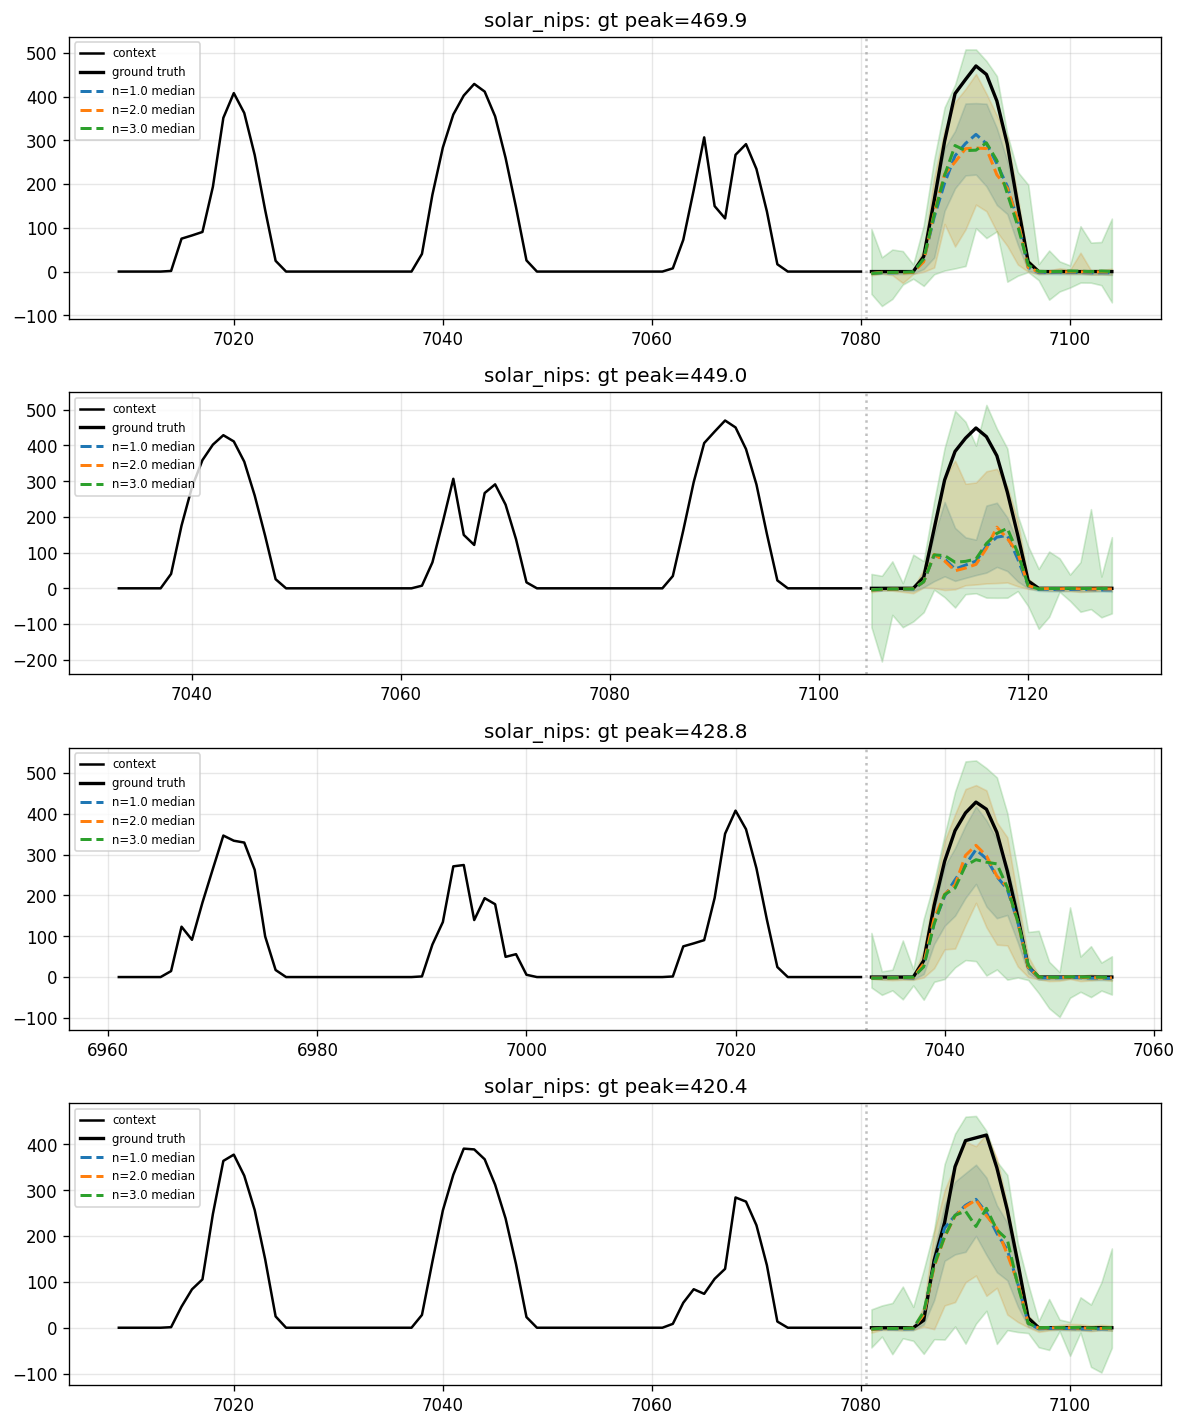
\includegraphics[width=0.99\linewidth]{figs/trajectories_solar.png}
\caption{Four highest-peak solar test windows. Dashed: median
forecast at $n \in \{1.0, 2.0, 3.0\}$. Shaded: $5$--$95\%$ sample
band. Same trained model, three operating points, scalar $n$ at
inference.}
\label{fig:trajectories}
\end{figure}

\begin{figure}[t]
\centering
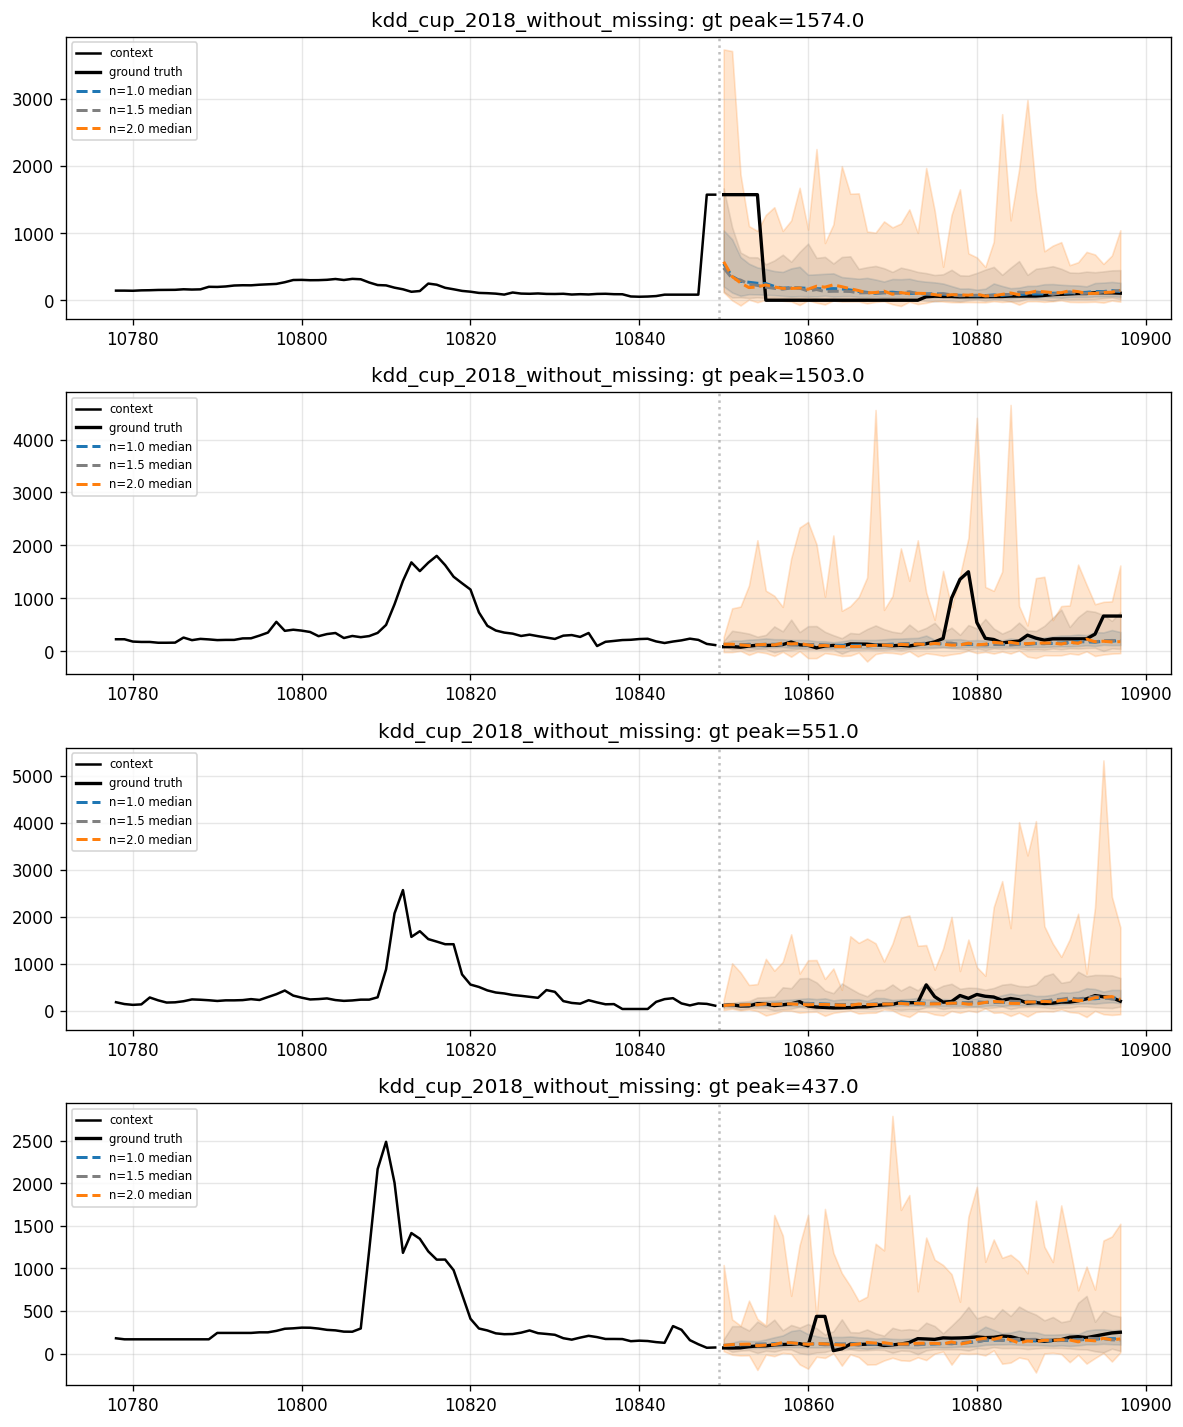
\includegraphics[width=0.99\linewidth]{figs/trajectories_kdd.png}
\caption{Same as Fig.~\ref{fig:trajectories} on KDD Cup 2018
air-quality pollution spikes (event-driven, unlike the periodic solar
case).}
\label{fig:trajectories-kdd}
\end{figure}

\subsection{CFG ablation}
\label{sec:cfg-ablation}

As a sanity check that classifier-free guidance with a learned
extremity adapter is \emph{not} a better dial, we trained a zero-init
extremity adapter on top of the v4 backbone conditioned on
$q = \operatorname{QuantileMap}(s(x))$ where $s(x) = \max|x|/\overline{|x|}$
is the peak-to-mean ratio (as advocated by Allen et
al.~\cite{allen2025tail}). With CFG dropout $0.1$ and $150$ epochs of
joint fine-tuning (unfrozen base, lr $10^{-4}$), the mean sample
maximum on solar grows from $211.6$ at $w{=}0$ to $236.9$ at $w{=}6$
($12\%$ dynamic range). Meanwhile twCRPS$_{0.99}$ grows (worse) from
$0.488$ to $0.511$: the CFG-scaled samples have larger peaks but are
farther from the data on the upper tail. Noise scaling on the same
backbone gives a larger dynamic range (sample max $196 \to 237$, $21\%$)
\emph{and} improves twCRPS$_{0.99}$ monotonically. We therefore do
not use CFG in the main pipeline.

\section{Discussion and Limitations}
\label{sec:discussion}

\paragraph{TSFlow tail advantage on solar.} TSFlow's GP-prior
starting distribution encodes temporally-correlated noise that our
isotropic Gaussian cannot replicate by scalar widening. On solar
twCRPS$_{0.99}$ this produces a genuine $19\%$ gap. An obvious
extension is to use a GP starting distribution at inference
instead of $\mathcal{N}(0, n^2 I)$, and we believe the inference-time
GP scale would recover the full tail-sharpness advantage at one-NFE
cost; we leave this to future work.

\paragraph{Exchange degeneracy.} The train-marginal $Q_{0.95}$ and
$Q_{0.99}$ thresholds for exchange rate land above nearly all test
samples, collapsing twCRPS to $\approx 0$ for every method. This is
not a failure of our evaluation code but a property of exchange rate
as a tail benchmark. We include the row for completeness.

\paragraph{Seed variance and uncertainty.} Our numbers in
Tables~\ref{tab:leaderboard}, \ref{tab:tail}, and~\ref{tab:kdd} are
single-training-seed, single-evaluation-seed point estimates with
$s \in \{100, 200, 500\}$ Monte Carlo samples per forecast. Within
the scales of the comparisons we make, differences on the order of
$0.5\%$ CRPS or $0.01$ twCRPS could be within seed noise. The
$+58\%$ Winkler and $+13$-point coverage deficits on TSFlow solar are
large enough to be robust to this, as is the bootstrap / seasonal
naïve comparison on KDD.

\paragraph{Reproducibility of TSFlow.} Our TSFlow rerun under
pure-PyTorch S4 kernels reaches CRPS $0.4701$ on solar vs the
published $0.343$ ($37\%$ gap). We caveat every tail-metric comparison
against TSFlow with this reproducibility uncertainty.

\paragraph{Missing external learned baselines.} Beyond TSFlow we have
not retrained TSDiff, TimeGrad, or TimeFlow under our metric code.
EVL~\cite{ding2019evl} has not been run. A future version should
include these at least on solar and KDD.

\paragraph{Novelty relative to DDIM-$\eta$ and temperature sampling.}
We recognize that starting-distribution width modifications are
familiar from DDIM~\cite{ddim}, BigGAN truncation~\cite{biggan}, and
language-model temperature. What we add is the specific empirical
claim that a single-scalar starting-variance modification is
\emph{sufficient} as the full body--tail dial in probabilistic
time-series forecasting, and that it matches the best operating point
of a Wessel-style twCRPS retrain family on the Pareto frontier.

\section{Conclusion}
\label{sec:conclusion}

A one-step MeanFlow forecaster trained with standard JVP
self-consistency exposes the full body--tail trade-off as a single
inference-time scalar---the noise scale of the starting Gaussian. On
the four NIPS4 benchmarks, TailFlow matches or beats TSFlow on every
standard and tail-weighted metric except solar twCRPS$_{0.99}$ (where
TSFlow's GP prior wins), with $32\times$ fewer NFEs and
$32\times$ lower wall-clock inference latency on matched backbones.
On a heavy-tailed KDD air-quality benchmark, it halves the $95\%$
Winkler interval score of a strong bootstrap baseline with correct
coverage. Against a twCRPS-retrained family the inference-time dial
reaches the same Pareto frontier for free. The practitioner's
workflow is: train once, validation-select the noise scale for the
application, deploy.

\bibliographystyle{plainnat}
\begin{thebibliography}{99}

\bibitem{geng2025meanflow}
Z.~Geng, M.~Deng, X.~Bai, J.~Z. Kolter, and K.~He.
\newblock Mean flows for one-step generative modeling.
\newblock {\em arXiv preprint arXiv:2505.13447}, 2025.

\bibitem{tsflow}
M.~Kollovieh, M.~Lienen, D.~L\"udke, L.~Schwinn, and S.~G\"unnemann.
\newblock Flow matching with {G}aussian process priors for probabilistic
  time series forecasting.
\newblock In {\em International Conference on Learning Representations},
  2025.

\bibitem{s4d}
A.~Gu, K.~Goel, and C.~R{\'e}.
\newblock On the parameterization and initialization of diagonal state
  space models.
\newblock In {\em NeurIPS}, 2022.

\bibitem{revin}
T.~Kim, J.~Kim, Y.~Tae, C.~Park, J.-H. Choi, and J.~Choo.
\newblock Reversible instance normalization for accurate time-series
  forecasting against distribution shift.
\newblock In {\em ICLR}, 2022.

\bibitem{ho2021cfg}
J.~Ho and T.~Salimans.
\newblock Classifier-free diffusion guidance.
\newblock In {\em NeurIPS Workshop}, 2021.

\bibitem{ddim}
J.~Song, C.~Meng, and S.~Ermon.
\newblock Denoising diffusion implicit models.
\newblock In {\em ICLR}, 2021.

\bibitem{biggan}
A.~Brock, J.~Donahue, and K.~Simonyan.
\newblock Large scale {GAN} training for high fidelity natural image
  synthesis.
\newblock In {\em ICLR}, 2019.

\bibitem{gneiting2011weighted}
T.~Gneiting and R.~Ranjan.
\newblock Comparing density forecasts using threshold- and
  quantile-weighted scoring rules.
\newblock {\em Journal of Business \& Economic Statistics},
  29(3):411--422, 2011.

\bibitem{allen2025tail}
S.~Allen, J.~Ziegel, and D.~Ginsbourger.
\newblock Tail calibration of probabilistic forecasts.
\newblock {\em Journal of the American Statistical Association},
  2025. arXiv:2407.03167.

\bibitem{wessel2025tail}
J.~Wessel and colleagues.
\newblock Enforcing tail calibration when training probabilistic
  forecast models.
\newblock {\em arXiv preprint arXiv:2506.13687}, 2025.

\bibitem{timegrad}
K.~Rasul, C.~Seward, I.~Schuster, and R.~Vollgraf.
\newblock Autoregressive denoising diffusion models for multivariate
  probabilistic time series forecasting.
\newblock In {\em ICML}, 2021.

\bibitem{csdi}
Y.~Tashiro, J.~Song, Y.~Song, and S.~Ermon.
\newblock {CSDI}: Conditional score-based diffusion models for
  probabilistic time series imputation.
\newblock In {\em NeurIPS}, 2021.

\bibitem{sssd}
J.~M.~L. Alcaraz and N.~Strodthoff.
\newblock Diffusion-based time series imputation and forecasting with
  structured state space models.
\newblock {\em TMLR}, 2023.

\bibitem{tsdiff}
M.~Kollovieh, A.~F. Ansari, M.~Bohlke-Schneider, J.~Zschiegner,
  H.~Wang, and Y.~Wang.
\newblock Predict, refine, synthesize: Self-guiding diffusion models
  for probabilistic time series forecasting.
\newblock In {\em NeurIPS}, 2023.

\bibitem{ding2019evl}
D.~Ding, M.~Zhang, X.~Pan, M.~Yang, and X.~He.
\newblock Modeling extreme events in time series prediction.
\newblock In {\em KDD}, 2019.

\end{thebibliography}

\end{document}
